%! TEX root = ../thesis.tex
\section{Linux Kernel}
\label{pps:sec:linux}

In this section, we apply the \interank{} model to the Linux kernel project, a well-known open-source software project.
In contrast to Wikipedia, most contributors to the Linux kernel are highly skilled professionals who dedicate a significant portion of their time and efforts to the project.

\subsection{Background \& Dataset}

The Linux kernel has fundamental impact on technology as a whole.
In fact, the Linux operating system runs 90\% of the cloud workload and 82\% of the smartphones~\citep{corbet2017linux}.
To collectively improve the source code, developers submit bug fixes or new features in the form of a \emph{patch} to collaborative repositories.
Review and integration time depend on the project's structure, ranging from a few hours or days for Apache Server~\citep{rigby2008open} to a couple of months for the Linux kernel~\citep{jiang2013will}.
In particular for the Linux kernel, developers submit patches to subsystem mailing lists, where they undergo several rounds of reviews.
After suggestions are implemented and if the code is approved, the patch can be committed to the subsystem maintainer's software repository.
Integration conflicts are spotted at this stage by other developers monitoring the maintainer's repository and any issues must be fixed by the submitter.
If the maintainer is satisfied with the patch, she commits it to Linus Torvalds' repository, who decides to include it or not with the next Linux release.

\subsubsection{Dataset Preprocessing}

We use a dataset collected by~\citet{jiang2013will} which spans Linux development activity between 2005 and 2012.
It consists of \num{670533} patches described using \num{62} features derived from e-mails, commits to software repositories, the developers' activity and the content of the patches themselves.
\citeauthor{jiang2013will} scraped patches from the various mailing lists and matched them with commits in the main repository.
In total, they managed to trace back 75\% of the commits that appear in Linus Torvalds' repository to a patch submitted to a mailing list.
A patch is labeled as \emph{accepted} ($q = 1$) if it eventually appears in a release of the Linux kernel, and \emph{rejected} ($q = 0$) otherwise.
We remove data points with empty subsystem and developer names, as well as all subsystems with no accepted patches.
Finally, we chronologically order the patches according to their mailing list submission time.

After preprocessing, the dataset contains $K= \num{619419}$ patches proposed by $ N = \num{9672} $ developers on $M = \num{394}$ subsystems.
34.12\% of these patches are accepted.
We then split the data into training set containing the first 80\% of patches and a validation set containing the remaining 20\%.

\subsubsection{Subsystem-Developer Correlation}

Given the highly complex nature of the project, one could believe that developers tend to specialize in few, independent subsystems.
Let $X_u = \{ X_{ui} \}_{i=1}^M$ be the collection of binary variables $ X_{ui} $ indicating whether developer $u$ has an accepted patch in subsystem $i$.
We compute the sample Pearson correlation coefficient $r_{uv} = \rho(X_u, X_v)$ between $X_u$ and $X_v$.
We show in Figure~\ref{pps:fig:linux_correlation} the correlation matrix $ \bm{R} = [r_{uv}] $ between developers patching subsystems.
Row $\bm{r}_u$ corresponds to developer $u$, and we order all rows according to the subsystem each developer $u$ contribute to the most.
We order the subsystems in decreasing order by the number of submitted patches, such that larger subsystems appear at the top of the matrix $\bm{R}$.
Hence, the blocks on the diagonal roughly correspond to subsystems and their size represents the number of developers involved with the subsystem.
As shown by the blocks, developers tend to specialize into one subsystem.
However, as the numerous non-zero off-diagonal entries reveal, they still tend to contribute substantially to other subsystems.
Finally, as highlighted by the dotted, blue square, subsystems number three to six on the diagonal form a cluster.
In fact, these four subsystems (\texttt{include/linux}, \texttt{arch/x86}, \texttt{kernel} and \texttt{mm}) are core subsystems of the Linux kernel.

\begin{figure}
	\centering
	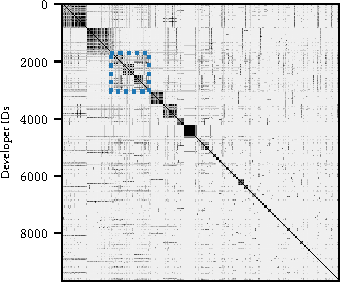
\includegraphics{pps-correlation-matrix}
	\caption{Correlation matrix $ \bm{R} $ between developers ordered according to the subsystem they contribute to the most. The blocks on the diagonal correspond to subsystems.
		Core subsystems form a strong cluster (blue square).}
	\label{pps:fig:linux_correlation}
\end{figure}

\subsection{Evaluation}

We consider the task of predicting whether a patch will be integrated into a release of the kernel.
Similarly to Section~\ref{pps:sec:wikipedia}, we use \interank{basic} and \interank{full} with $D = 20$ latent dimensions to learn the developers' skills, the subsystems' difficulty, and the interaction between them.

\subsubsection{Competing Approaches}
Three baselines that we consider---\emph{average}, \emph{user-only} and \emph{GLAD}---are identical to those described in Section~\ref{pps:sec:wikicompeting}.
In addition, we also compare our model to a random forest classifier trained on domain-specific features similar to the one used by~\citet{jiang2013will}.
In total, this classifier has access to 21 features for each patch.
Features include information about the developer's experience up to the time of submission (e.g., number of accepted commits, number of patches sent), the e-mail thread (e.g., number of developers in copy of the e-mail, size of e-mail, number of e-mails in thread until the patch) and the patch itself (e.g., number of lines changed, number of files changed).
We optimize the hyperparameters of the random forest using a grid-search.
As the model has access to domain-specific features about each edit, it is representative of the class of specialized methods tailored to the Linux kernel peer-production system.

\subsubsection{Results}

Table~\ref{pps:tab:linux_results} displays the average log-likelihood and area under the precision-recall curve (AUPRC).
\interank{full} performs best in terms of both metrics.
In terms of AUPRC, it outperforms the random forest classifier by 4.4\%, GLAD by 5\%, and the \emph{user-only} baseline by 7.3\%.

\begin{table}
	\centering
	\caption{Predictive performance on the \emph{accepted patch} classification task for the Linux kernel.
		The best performance is highlighted in bold.}
	\label{pps:tab:linux_results}
	\begin{tabular}{lrr}
		\toprule
		Model            & Avg. log-likelihood & AUPRC          \\
		\midrule
		\interank{basic} & -0.589              & 0.525          \\
		\interank{full}  & \textbf{-0.588}     & \textbf{0.527} \\
		\addlinespace
		Average          & -0.640              & 0.338          \\
		User-only        & -0.601              & 0.491          \\
		GLAD             & -0.598              & 0.502          \\
		Random forest    & -0.599              & 0.505          \\
		\bottomrule
	\end{tabular}
\end{table}

We show the precision-recall curves in Figure~\ref{pps:fig:linux_results}.
Both \interank{full} and \interank{basic} perform better than the four baselines.
Notably, they outperform the random forest in the high-precision regime, even though the random forest uses content-based features about developers, subsystems and patches.
In the high-recall regime, the random forest attains a marginally better precision.
The \emph{user-only} and GLAD baselines perform worse than all non-trivial models.

\begin{figure}
	\centering
	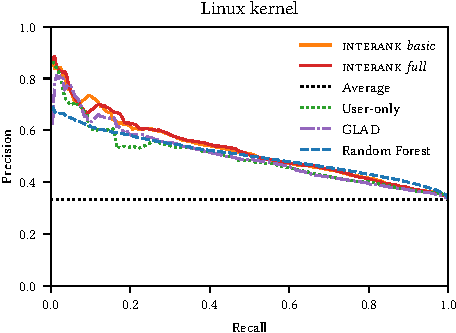
\includegraphics[width=\linewidth*3/4]{pps-linux-pr}
	\caption{Precision-recall curves on the bad edit classification task for the Linux kernel. \textsc{interank} (solid orange and red) outperforms the user-only baseline (dotted green), the random forest classifier (dashed blue), and GLAD (dash-dotted purple).}
	\label{pps:fig:linux_results}
\end{figure}

\subsection{Interpretation of Model Parameters}

We show in Table~\ref{pps:tab:linux_subsystems} the top-five and bottom-five subsystems according to  difficulties $\{d_i\}$ learned by \interank{full}.
We note that even though patches submitted to difficult subsystems have in general low acceptance rate, \interank{} enables a finer ranking by taking into account \emph{who} is contributing to the subsystems.
This effect is even more noticeable with the five subsystems with smallest difficulty value.

The subsystems $i$ with largest $d_i$ are \emph{core} components, whose integrity is crucial to the system.
For instance, the \texttt{usr} subsystem, providing code for RAM-related instructions at booting time, has barely changed in the last seven years.
On the other hand, the subsystems $i$ with smallest $d_i$ are \textit{peripheral} components serving specific devices, such as digital signal processors or gaming consoles.
These components can arguably tolerate a higher rate of bugs, and hence they evolve more frequently.

\begin{table}
	\centering
	\caption{Top-five and bottom-five subsystems according to their difficulty $d_i$.}
	\label{pps:tab:linux_subsystems}
	\begin{tabular}{llrrr}
		\toprule
		Difficulty & Subsystem                  & \% Acc. & \# Patch & \# Dev. \\
		\midrule
		+2.664     & \texttt{usr}               & 1.88\%  & 796      & 70      \\
		+1.327     & \texttt{include}           & 7.79\%  & 398      & 101     \\
		+1.038     & \texttt{lib}               & 15.99\% & 5642     & 707     \\
		+1.013     & \texttt{drivers/clk}       & 34.34\% & 495      & 81      \\
		+0.865     & \texttt{include/trace}     & 17.73\% & 547      & 81      \\
		\midrule
		-1.194     & \texttt{drivers/addi-data} & 78.31\% & 272      & 8       \\
		-1.080     & \texttt{net/tipc}          & 43.11\% & 573      & 44      \\
		-0.993     & \texttt{drivers/ps3}       & 44.26\% & 61       & 9       \\
		-0.936     & \texttt{net/nfc}           & 73.04\% & 204      & 26      \\
		-0.796     & \texttt{arch/mn10300}      & 45.40\% & 359      & 63      \\
		\bottomrule
	\end{tabular}
\end{table}

\citet{jiang2013will} establish that a high prior subsystem churn (\textit{i.e.}, high number of previous commits to a subsystem) leads to lower acceptance rate.
We approximate the number of commits to a subsystem as the number of patches submitted multiplied by the subsystem's acceptance rate.
The first quartile of subsystems according to their increasing difficulty, \textit{i.e.}, the least difficult subsystems, has an average churn of \num{687}.
The third quartile, \textit{i.e.}, the most difficult subsystems, has an average churn of \num{833}.
We verify hence that higher churn correlates with difficult subsystems.
This corroborates the results obtained by~\citeauthor{jiang2013will}

As shown in Figure~\ref{pps:fig:linux_results}, if false negatives are not a priority, \interank{} will yield a substantially higher precision.
In other words, if the task at hand requires that the patches classified as accepted are actually the ones integrated in a future release, then \interank{} will yield more accurate results.
For instance, it would be efficient in supporting Linus Torvalds in the development of the Linux kernel by providing him with a restricted list of patches that are likely to be integrated in the next release of the Linux kernel.
